\documentclass[12pt]{report}
\usepackage[utf8]{inputenc}
\usepackage[russian]{babel}
%\usepackage[14pt]{extsizes}
\usepackage{listings}

% Для листинга кода:
\lstset{ %
language=go,                 % выбор языка для подсветки 
basicstyle=\small\sffamily, % размер и начертание шрифта для подсветки кода
numbers=left,               % где поставить нумерацию строк (слева\справа)
numberstyle=\tiny,           % размер шрифта для номеров строк
stepnumber=1,                   % размер шага между двумя номерами строк
numbersep=5pt,                % как далеко отстоят номера строк от подсвечиваемого кода
showspaces=false,            % показывать или нет пробелы специальными отступами
showstringspaces=false,      % показывать или нет пробелы в строках
showtabs=false,             % показывать или нет табуляцию в строках            
tabsize=2,                 % размер табуляции по умолчанию равен 2 пробелам
captionpos=t,              % позиция заголовка вверху [t] или внизу [b] 
breaklines=true,           % автоматически переносить строки (да\нет)
breakatwhitespace=false, % переносить строки только если есть пробел
escapeinside={\#*}{*)}   % если нужно добавить комментарии в коде
}

% Для измененных титулов глав:
\usepackage{titlesec, blindtext, color} % подключаем нужные пакеты
\usepackage{float}
\newcommand{\hsp}{\hspace{20pt}} % длина линии в 20pt
% titleformat определяет стиль
\titleformat{\chapter}[hang]{\Huge\bfseries}{\thechapter\hsp\textcolor{gray75}{|}\hsp}{0pt}{\Huge\bfseries}


% plot
\usepackage{pgfplots}
\usepackage{filecontents}
\usepackage{amsmath}
\usepackage{tikz,pgfplots}
\usetikzlibrary{datavisualization}
\usetikzlibrary{datavisualization.formats.functions}
\begin{filecontents}{parallel.dat}
10   2.6328
20 4.6109
30 6.62439
50 10.62628
\end{filecontents}
\begin{filecontents}{linear.dat}
10  6.0138
20 12.0312
30 18.0679
50 30.06836
\end{filecontents}

\usepackage{graphicx}
\graphicspath{{src/}}
\DeclareGraphicsExtensions{.pdf,.png,.jpg}

\begin{document}
%\def\chaptername{} % убирает "Глава"
\begin{titlepage}
	\centering
	{\scshape\LARGE МГТУ им. Баумана \par}
	\vspace{3cm}
	{\scshape\Large Лабораторная работа №5\par}
	\vspace{0.5cm}	
	{\scshape\Large По курсу: "Анализ алгоритмов"\par}
	\vspace{1.5cm}
	{\huge\bfseries Конвеерная обработка\par}
	\vspace{2cm}
	\Large Работу выполнил: Мокеев Даниил, ИУ7-54\par
	\vspace{0.5cm}
	\Large Преподаватели:  Волкова Л.Л., Строганов Ю.В.\par

	\vfill
	\large \textit {Москва, 2019} \par
\end{titlepage}

\tableofcontents

\newpage
\chapter*{Введение}
\addcontentsline{toc}{chapter}{Введение}

Цель работы: изучение возможности конвеерной обработки и использование такого подхода на практике. Необходимо сравнить времени работы алгоритма на нескольких потоков и линейную реализацию.

В ходе лабораторной работы предстоит:
\begin{itemize}
	\item Реализовать конвейер на потоках; 
	\item Реализовать линейную обработку; 
	\item Провести сравнение времени работы;
\end{itemize}

\chapter{Аналитическая часть}
Ковейер - система поточного производства. В терминах программирования ленты конвейера представленны функциями, выполняющими над неким набором данных операции и предающие их на следующую ленту конвейера. Моделирование конвейерной обработки хорошо сочетается с технологией многопоточного программирования - под каждую ленту конвейера выделяется отдельный поток, все потоки работают в ассинхронном режиме.
В качестве предметной области я решил выбрать торты - на первой линии конвейера замешивается тесто, на второй наносят глазурь, на третьей декорируют.


\section{Параллельное программирование}

При использовании многопроцессорных вычислительных систем с общей памятью обычно предполагается, что имеющиеся в составе системы процессоры обладают равной производительностью, являются равноправными при доступе к общей памяти, и время доступа к памяти является одинаковым (при одновременном доступе нескольких процессоров к одному и тому же элементу памяти очередность и синхронизация доступа обеспечивается на аппаратном уровне). Многопроцессорные системы подобного типа обычно именуются симметричными мультипроцессорами (symmetric multiprocessors, SMP).

Перечисленному выше набору предположений удовлетворяют также активно развиваемые в последнее время многоядерные процессоры, в которых каждое ядро представляет практически независимо функциони рующее вычислительное устройство.

Обычный подход при организации вычислений для многопроцессорных вычислительных систем с общей памятью – создание новых параллельных методов на основе обычных последовательных программ, в которых или автоматически компилятором, или непосредственно программистом выделяются участки независимых друг от друга вычислений. Возможности автоматического анализа программ для порождения параллельных вычислений достаточно ограничены, и второй подход является преобладающим. При этом для разработки параллельных программ могут применяться как новые алгоритмические языки, ориентированные на параллельное программирование, так и уже имеющиеся языки, расширенные некоторым набором операторов для параллельных вычислений.

Широко используемый подход состоит и в применении тех или иных библиотек, обеспечивающих определенный программный интерфейс (application programming interface, API) для разработки параллельных программ. В рамках такого подхода наиболее известны Windows Thread API. Однако первый способ применим только для ОС семейства Microsoft Windows, а второй вариант API является достаточно трудоемким для использования и имеет низкоуровневый характер \cite{Barkalov}.

\subsection{Организация взаимодействия параллельных потоков}
Потоки исполняются в общем адресном пространстве параллельной программы. Как результат, взаимодействие параллельных потоков можно организовать через использование общих данных, являющихся доступными для всех потоков. Наиболее простая ситуация состоит в использовании общих данных только для чтения. В случае же, когда общие данные могут изменяться несколькими потоками, необходимы специальные усилия для организации правильного взаимодействия.

\section{Вывод}
Была рассмотрена конвейерная обработка данных, технология параллельного программирования и
организация взаимодействия параллельных потоков.

\chapter{Конструкторская часть}
\textbf{Требования к вводу:}
На ввод подается целое число - желаемое колличество изготовленных экземпляров
\newline
\textbf{Требования к программе:}
\begin{itemize}
	\item вывод статистики обаботанных экземпляров;
	\item при матрицах неправильных размеров программа не должна аварийно завершаться.
\end{itemize}

\section{Схемы алгоритмов}
В данной части будет рассмотрена схема алгоритма.

\section{Распараллеливание программы}
Распрараллеливание программы должно ускорять время работы. Это достигается за счет перенесения каждой из лент конвейера на отдельный поток.

\section{Вывод}
В данном разделе была рассмотрена схема алгоритма и способ ее распараллеливания.

\chapter{Технологическая часть}
\section{Выбор ЯП}
Я выбрал в качестве языка программирования Golang, потому как он достаточно удобен, быстр и успешно использует концепции мультипоточного программирования.

Время работы алгоритмов было замерено с помощью функции Now() из библиотеки time.

\section{Описание структуры ПО}
\begin{figure}[!htbp]
	\centering
	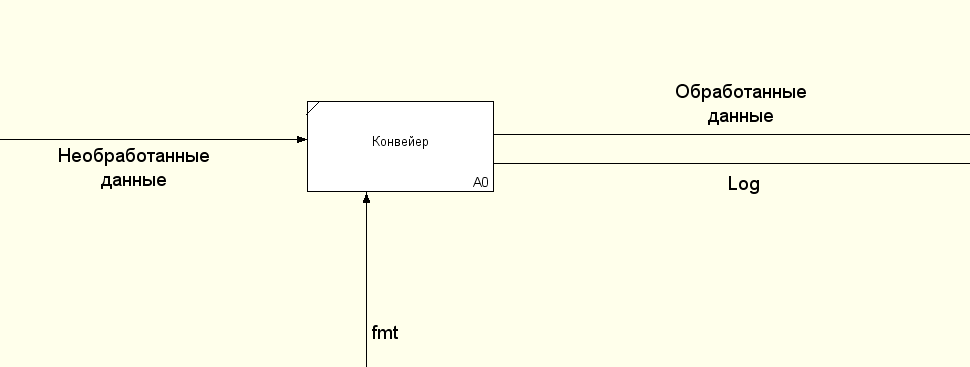
\includegraphics[width=1.25\linewidth]{lab05ram}
	\caption{Функциональная схема умножения матриц (IDEF0 диаграмма 1 уровня)}
	\label{fig:mpr}
\end{figure}

\section{Сведения о модулях программы}
Программа состоит из:
\begin{itemize}
	\item lab05.go- главный файл программы, в котором располагается точка входа в программу.
	\item linear.go - файл, содержащий функцию линейной обработки данных.
\end{itemize}

\section{Листинг кода алгоритмов}

\begin{lstlisting}[label=CodeStand,caption = Параллельный конвейер]
func conv(amount int, wait chan int) *queue{
	uno := make(chan *cake, 5)
	dos := make(chan *cake, 5)
	tres := make(chan *cake, 5)
	line := new_queue(amount) 
	first := func(){
		for{
			select{
			case a := <- uno:
			a.dough = true
			
			a.started_dough = time.Now()
			took_dough := 200
			time.Sleep(time.Duration(took_dough) * time.Millisecond)
			
			a.finished_dough = time.Now()
			dos <- a
			}
		}
	}
	
	second:= func(){
	for{
		select{
			case a := <- dos:
			//fmt.Printf("Cake num %d started topping\n", a.num)
			a.topping = true
			
			a.started_topping = time.Now()
			took_topping := 200
			time.Sleep(time.Duration(took_topping) * time.Millisecond)
			
			a.finished_topping = time.Now()
			tres <- a
			}
		}
	}
	
	third := func(){
		for{
			select{
			case a := <- tres:
			//fmt.Printf("Cake num %d started decor\n", a.num)
			a.decor = true
			
			a.started_decor = time.Now()
			took_decor := 200
			time.Sleep(time.Duration(took_decor) * time.Millisecond)
			
			a.finished_decor = time.Now()
			line.push(a)
			if (a.num == amount){
			wait <- 0 }
			
			}
		}
	}
	
	go first()
	go second()
	go third()
	for i:=0; i<=amount; i++{
		a := new(cake)
		a.num = i
		uno <- a
	}
	return line
}
\end{lstlisting}

\begin{lstlisting}[label=winograd_mult,caption=Линейный конвейер]
func linear (amount int)*queue{
	queue_for_topping := new_queue(amount)
	queue_for_decor := new_queue(amount)
	finished := new_queue(amount)
	i:= 0
	for ;i!=-1;{
		a := new(cake)
		a.num = i
		first(a, queue_for_topping)
		if queue_for_topping.last >= 0{
			second(queue_for_topping.pop(), queue_for_decor)
		}
		if queue_for_decor.last >= 0{
			third(queue_for_decor.pop(), finished)
		}
		if finished.waiting[len(finished.waiting)-1] != nil{
			return finished}
		i+=1
	}
	return finished
}
\end{lstlisting}

\section{Вывод}
В данном разделе была рассмотрена структура ПО и листинги кода программы.

\chapter{Исследовательская часть}
Был проведен замер времени работы алгоритмов с использованием разного колличества изготавливаемых изделий.
Исследования были проведены на процессоре Intel Core i5-6200U
На каждом ковейре время производства занимало 0.2сек
\section{Примеры работы}
\begin{figure}[H]
	\center{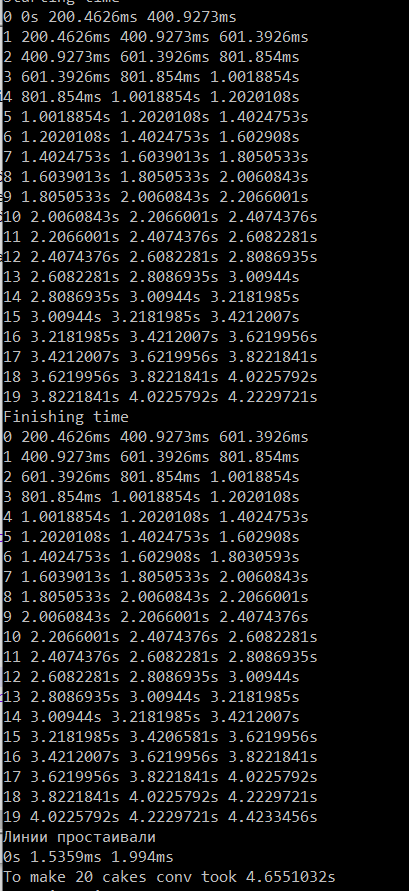
\includegraphics[scale=1.1]{example_threads.png}} 
	\caption{Пример работы программы - конефейер на потоках}
	\label{ris:example_th}
\end{figure}
\begin{figure}[H]
	\center{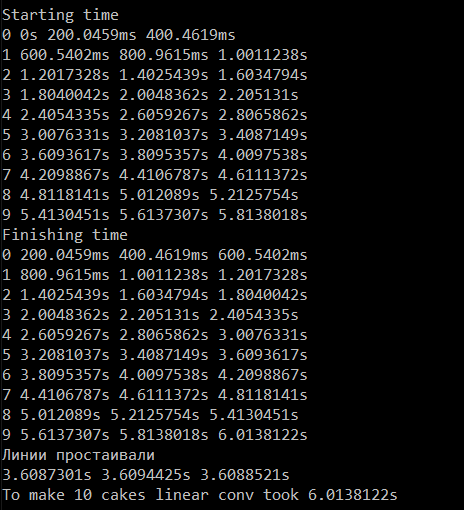
\includegraphics[scale=1.1]{example_linear.png}} 
	\caption{Пример работы программы - линейная обработка данных и результат}
	\label{ris:example_lin}
\end{figure}

\section{Постановка эксперемента}
Проведем сравнение для каждого из алгоритмов. Для замера времени будем использовать функцию time.Now()

Сравним результаты для линейной обработки данных и распараллеленой:
\newpage

\begin{figure}
\begin{tikzpicture}[thick, scale=1.4]
\begin{axis}[
    	axis lines = left,
    	xlabel = $size$,
    	ylabel = {$time(sec)$},
	legend pos=north west,
	ymajorgrids=true
]
\addplot[color=red] table[x index=0, y index=1] {parallel.dat}; 
\addplot[color=green] table[x index=0, y index=1] {linear.dat};

\addlegendentry{Ассинхронный конвейер}
\addlegendentry{Синхронный конвейер}
\end{axis}
\end{tikzpicture}
\caption{Сравнение параллельного и обычного алгоритмов} \label{plot:even}
\end{figure}
\par

\newpage
\subsection{Заключение эксперементальной части}
Экперемент показывает, что использование нескольких потоков для реализации конвейерной обработки данных ускоряет алгоритм в несколько раз. При этом возникает ситуация при которой ленты не простаивают. Тратится лишь малое время для передачи данных на линию.
\chapter*{Заключение}
\addcontentsline{toc}{chapter}{Заключение}
В ходе лабораторной работы были изучены возможности параллельных вычислений, реализован алгоритм конвейерной обработки данных
с помощью параллельных вычислений.

Было проведено сравнение синхронной версии того же алгоритма и ассинхронной. Выяснилось, что при использовании потоков, время работы алгоритма не просто сокращается, но и снижается скорость роста времени при увеличении числа изготавливаемых экземпляров.

\addcontentsline{toc}{chapter}{Список литературы}
\begin{thebibliography}{3}
	\bibitem{Beloysov}
	И. В. Белоусов(2006), Матрицы и определители, учебное пособие по линейной алгебре, с. 1 - 16
	\bibitem{Gall2012}
	Le Gall, F. (2012), "Faster algorithms for rectangular matrix multiplication", Proceedings of the 53rd Annual IEEE Symposium on Foundations of Computer Science (FOCS 2012), pp. 514–523
	%https://arxiv.org/pdf/1204.1111.pdf
	\bibitem{Barkalov}
	Константин Баркалов, Владимир Воеводин, Виктор Гергель. Intel Parallel Programming [Электронный ресурс], - режим доступа https://www.intuit.ru/studies/courses/4447/983/lecture/14925
	\bibitem{Microsoft}
	Руководство по языку C\#[Электронный ресурс], - режим доступа: https://docs.microsoft.com/ru-ru/dotnet/csharp/
\end{thebibliography}

\end{document}

